\documentclass[main.tex]{subfiles}
\begin{document}

\subsection{Azure Quantum Basics} 

    The first step in using Azure Quantum is to create a \href{https://portal.azure.com/#create/Microsoft.AzureQuantum}{Quantum Workspace}. Once created the user can select from a set of quantum hardware providers including: IonQ, Quantinuum, and Microsoft Quantum-Inspired Optimization (QIO). IonQ provides the option to use either quantum simulation \texttt{ionq.simulator} with access to 29  simulated qubits or quantum processing unit hardware \texttt{ionq.qpu} with 11 IonQ trapped-ion qubits. The Q\# language is used to define the users quantum algorithm and is executed in Jupyter notebook cells running in the Quantum Workspace. A  \href{https://github.com/jwcrandall/csci-6907-quantum-computing-project/blob/main/hello-world-qsharp-ionq.ipynb}{Q\# hello world} program with IonQ hardware using Jupyter notebook cells is composed of connecting to the Azure Quantum workspace, building the quantum program, and submitting the quantum program to IonQ. Once IonQ returns the result the user can visualize the output statistics using Python visualization tools, with \texttt{matplotlib} used in the linked example.
    
    %\begin{figure}
    %    \centering
    %    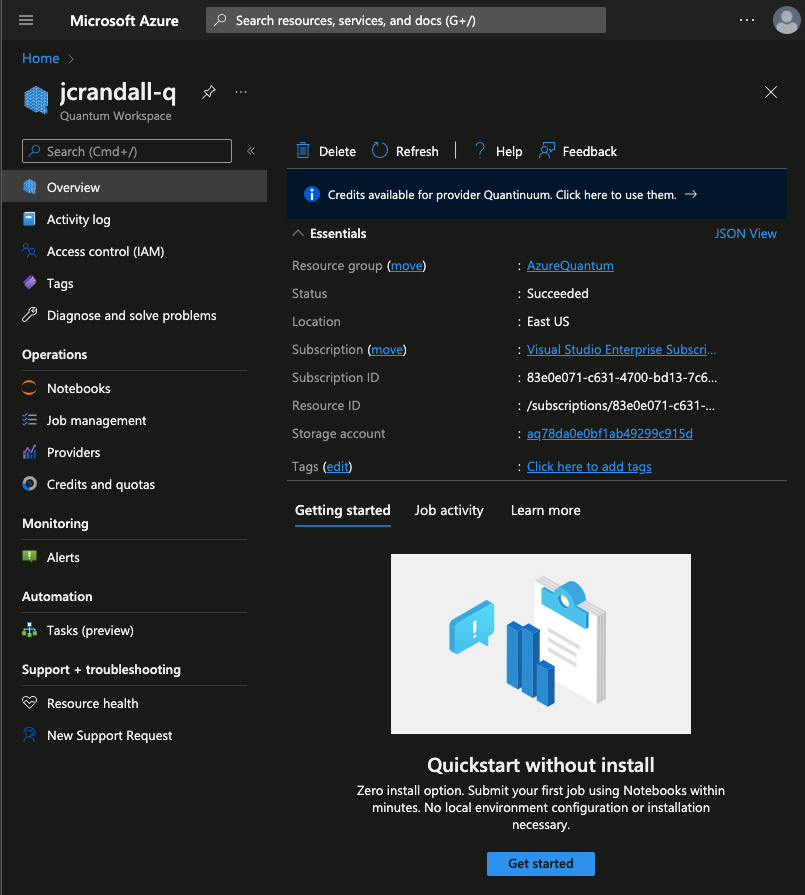
\includegraphics[width=4in]{paper/figs/quantumWorkspace.png}
    %        \caption{Quantum Workspace and Q# hello world statistics}
    %    \label{fig:quantumWorkspace}
    %\end{figure}

\subsection{Shor's Algorithm}

    This \href{https://github.com/jwcrandall/csci-6907-quantum-computing-project/blob/main/shors-algorithm.ipynb}{implementation} of Shor's algorithm uses $n=3$ IonQ trapped-ion qubits. Given: $M$, the numbers to be factored:
    
    \begin{itemize}
        \item Step 1: Pick $n$ qubits so that $N = 2^n > M$.
        \item Step 2: Pick a random $ a < M $.
        \item Step 3: If $\text{gcd}(a,M) \neq 1$, we've factored $M$, so stop.
        \item Step 4: If not, use $a$ and $M$ in the Figure \ref{fig:shorsCircuit} circuit and obtain an outcome for $|y\rangle$.
        \item Step 5: Find the close convergents of $\frac{y}{N}$, and thus a guess for $r$.
        \item Step 6: See if these two conditions are satisfied:
        \begin{itemize}
            \item $r$ is even.
            \item $a^{\frac{r}{2}} + 1 \equiv_M 0 $ is false, where $a \bmod M=b \bmod M$ is written as $a \equiv{ }_{M} b$
            \item If not, try a different Step 2 and repeat steps 3-6.
        \end{itemize}
        \item Step 7: If the conditions are satisfed, attempt to factor $M$ as shown via the numbers $a^{\frac{r}{2}} + 1$ and $a^{\frac{r}{2}} - 1$.
        \item Repeat as needed to try different $r$ so that at least one provides a $y$ near $\frac{N}{r}$.
    \end{itemize}

    \begin{figure}
        \centering
        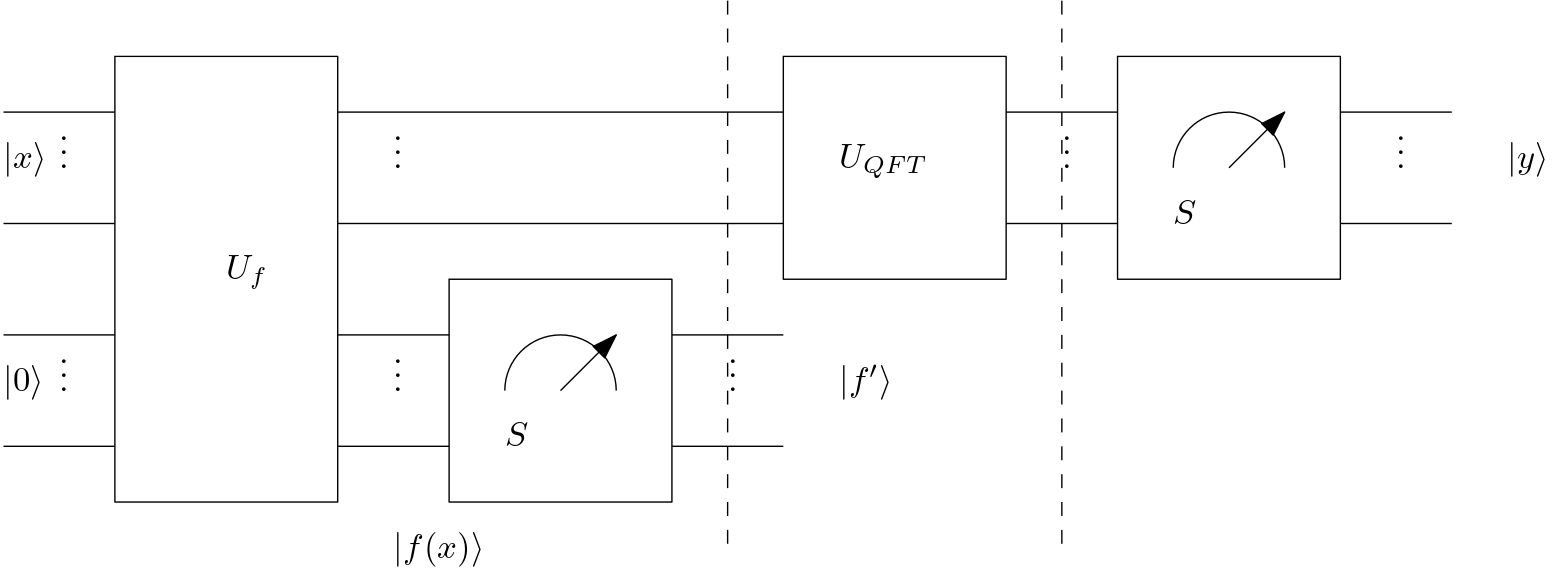
\includegraphics[width=6in]{paper/figs/shorsCircuit.png}
            \caption{Quantum circuit $U_f$ computes $f_{a,M}(x)$ for input $x$ where $f_{a,M}(x)=a^x \mod M$, where measurement of the $|f(x)\rangle$ values will result in one $|f^{\prime} \rangle$. After the first measurement the unitary Quantum Fourier Transform $U_{QFT}$, defined in Figure \ref{fig:3qQFT} for three qubits, occurs. The outcome from the post-QFT measurement results in one of the standard-basis $|y\rangle$ vectors as the outcome in the top-$n$ qubits}
        \label{fig:shorsCircuit}
    \end{figure}
    
     \begin{figure}
        \centering
        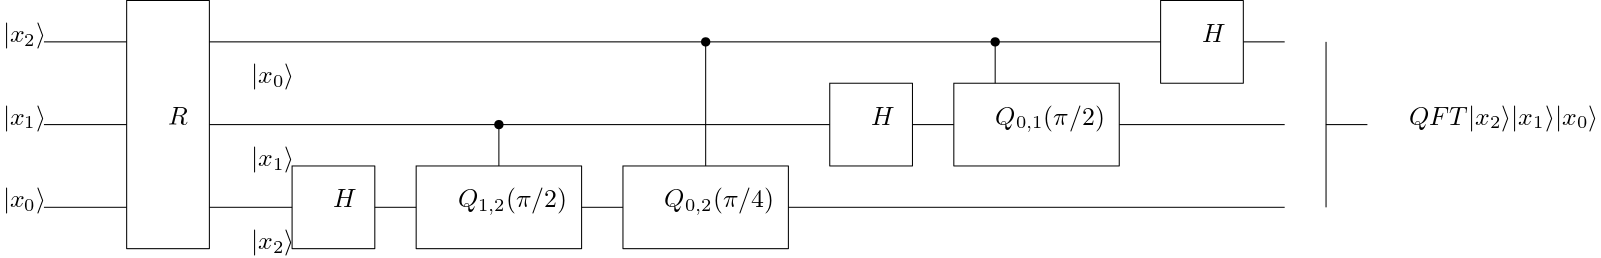
\includegraphics[width=7in]{paper/figs/3qQFT.png}
            \caption{Three Qubit Unitary Quantum Fourier Transform}
        \label{fig:3qQFT}
    \end{figure}
    
    
    

\end{document}